\documentclass[tikz]{standalone}
\usepackage{tikz,amsmath}
\usetikzlibrary{calc}
\begin{document}
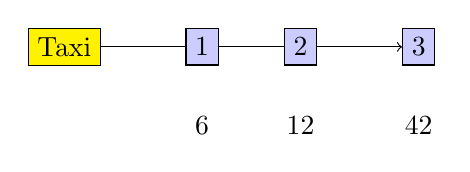
\begin{tikzpicture}
    \node (start) [draw,fill=yellow] {Taxi};
    \node (A) [draw,fill=blue!20!, right of=start, xshift=.75cm] {$1$};
    \node (B) [draw,fill=blue!20!, right of=start, xshift=2cm] {$2$};
    \node (C) [draw,fill=blue!20!, right of=start, xshift=3.5cm] {$3$};
    \node [below of=A] {6};
    \node [below of=B] {12};
    \node [below of=C] {42};
    \draw [->] (start) -- (A) -- (B) -- (C);
\end{tikzpicture}
\end{document}
